\documentclass[french, 12pt]{article}

\usepackage[utf8]{inputenc}    % Encodage
\usepackage[T1]{fontenc}       % Encodage des polices
\usepackage{lipsum}            % Générateur de texte pour les exemples
\usepackage{graphicx}          % Pour inclure des images
\usepackage{amsmath}           % Pour les formules mathématiques
\usepackage{amsfonts}          % Pour les polices mathématiques
\usepackage{amssymb}           % Pour les symboles mathématiques
\usepackage{hyperref}          % Pour les liens
\usepackage{fancyhdr}          % Pour les en-têtes et pieds de page

% Configuration de l'en-tête et du pied de page
\pagestyle{fancy}
\fancyhf{}
\fancyhead[L]{Sokoban}
\fancyhead[R]{Sacha David et Nathael Carlier}     
\fancyfoot[C]{\thepage}        

% Titre et auteur
\title{Projet Sokoban}
\author{Sacha David et Nathael Carlier\\
        Prép'Isima 2}
\date{\today}




% détaillant la modélisation du jeu (choix retenus pour la modélisation du plateau, 
%des éléments ainsi que les strutures de données. À des fins d’évaluations, il sera précisé comment lancer le programme.)
\begin{document}

\maketitle

\tableofcontents
    
\section{Introduction}

    Le but de ce projet est de recréer le jeu \href{https://fr.wikipedia.org/wiki/Sokoban}{Sokoban} en utilisant le language de programmation C. 

    C'est un jeu ou le joueur doit ranger des caisses sur des cases cibles. Il peut se déplacer dans les quatre directions, et seulement pousser (pas tirer) une seule caisse à la fois. Une fois toutes les caisses rangées, le niveau est réussi et le joueur passe au niveau suivant, plus difficile en général. L'idéal est de réussir avec le moins de déplacement possibles. En principe le personnage de ce jeu est un gardien d'entrepôt rangeant les caisses d'un entrepôt à leur bon endroit. Sokoban ressemble en général à l'illustration ci-dessus (mais comme vous allez le voir nous avons pris quelque liberter de design).

    \begin{figure}[h]
        \centering
        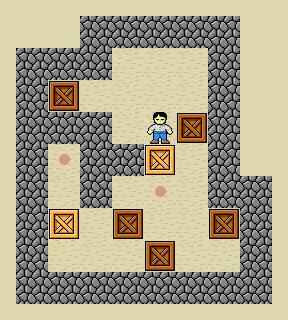
\includegraphics[width=0.4\textwidth]{illustration/base_sokoban.png}
        \caption{Exemple typique d'un jeu sokoban}
    \end{figure}

\section{Nécessaire pour le lancement du jeu}

Pour cette section on vous renvoie sur la \href{../doc/redirect.html}{page d'accueil} de notre documentation expliquant la démarche a suivre pour compiler et éxécuter le jeu.

\section{Choix de  modélisation} % Ou D.A. jsp pas quoi mettre 

    \subsection{Explication}
        Nous avons remarqué que les graphismes du jeu de base était trop basiques et pas forcément jolies. C'est pour cela que nous avons décider de complétement changer la direction artistique de notre jeu pour donner un cotê plus mignon au jeux.

    \subsection{Changements}
        Le personnage ne sera plus un gardien d'entrepôt mais un \href{https://fr.wikipedia.org/wiki/Hydrochoerus_hydrochaeris}{capybara} et lieu dans lequel le jeu ce déroule sera une étendu d'eau en bas d'une casquade. Notre personnage ne déplacera pas de caisse sur leur rangement mais il déplacera des oranges sur des nénuphars. 
        Deplus les murs en pierre n'existeront pas, ce sera des rochers dépassant de l'eau, le tout avec un rendu en isométrique.

        % Mettre image montrant la différence entre les deux




\section{Structuration des données}

    \subsection{Plateau de jeu}
    % Comment est gérer le plateau

    \subsection{Joueur}
    % Comment est gérer le joueur


\section{Affichage du jeu}
% Comment on affiche le tout 

\section{Conclusion}



\end{document}
